\documentclass[a4paper, 14pt]{extarticle}
\UseRawInputEncoding



% Поля
%--------------------------------------
\usepackage{geometry}
\geometry{a4paper,tmargin=2cm,bmargin=2cm,lmargin=3cm,rmargin=1cm}
%--------------------------------------


%Russian-specific packages
%--------------------------------------
\usepackage[T2A]{fontenc}
\usepackage[utf8]{inputenc} 
\usepackage[english, main=russian]{babel}
%--------------------------------------

\usepackage{textcomp}

% Красная строка
%--------------------------------------
\usepackage{indentfirst}               
%--------------------------------------             


%Graphics
%--------------------------------------
\usepackage{graphicx}
\graphicspath{ {./images/} }
\usepackage{wrapfig}
%--------------------------------------

% Полуторный интервал
%--------------------------------------
\linespread{1.3}                    
%--------------------------------------

%Выравнивание и переносы
%--------------------------------------
% Избавляемся от переполнений
\sloppy
% Запрещаем разрыв страницы после первой строки абзаца
\clubpenalty=10000
% Запрещаем разрыв страницы после последней строки абзаца
\widowpenalty=10000
%--------------------------------------

%Списки
\usepackage{enumitem}

%Подписи
\usepackage{caption} 

%Гиперссылки
\usepackage{hyperref}

\hypersetup {
	unicode=true
}

%Рисунки
%--------------------------------------
\DeclareCaptionLabelSeparator*{emdash}{~--- }
\captionsetup[figure]{labelsep=emdash,font=onehalfspacing,position=bottom}
%--------------------------------------

\usepackage{tempora}

%Листинги
%--------------------------------------
\usepackage{listings}
\lstset{
  basicstyle=\ttfamily\footnotesize, 
  %basicstyle=\footnotesize\AnkaCoder,        % the size of the fonts that are used for the code
  breakatwhitespace=false,         % sets if automatic breaks shoulbd only happen at whitespace
  breaklines=true,                 % sets automatic line breaking
  captionpos=t,                    % sets the caption-position to bottom
  inputencoding=utf8,
  frame=single,                    % adds a frame around the code
  keepspaces=true,                 % keeps spaces in text, useful for keeping indentation of code (possibly needs columns=flexible)
  keywordstyle=\bf,       % keyword style
  numbers=left,                    % where to put the line-numbers; possible values are (none, left, right)
  numbersep=5pt,                   % how far the line-numbers are from the code
  xleftmargin=25pt,
  xrightmargin=25pt,
  showspaces=false,                % show spaces everywhere adding particular underscores; it overrides 'showstringspaces'
  showstringspaces=false,          % underline spaces within strings only
  showtabs=false,                  % show tabs within strings adding particular underscores
  stepnumber=1,                    % the step between two line-numbers. If it's 1, each line will be numbered
  tabsize=2,                       % sets default tabsize to 8 spaces
  title=\lstname                   % show the filename of files included with \lstinputlisting; also try caption instead of title
}
%--------------------------------------

%%% Математические пакеты %%%
%--------------------------------------
\usepackage{amsthm,amsfonts,amsmath,amssymb,amscd}  % Математические дополнения от AMS
\usepackage{mathtools}                              % Добавляет окружение multlined
\usepackage[perpage]{footmisc}
%--------------------------------------

%--------------------------------------
%			НАЧАЛО ДОКУМЕНТА
%--------------------------------------

\begin{document}

%--------------------------------------
%			ТИТУЛЬНЫЙ ЛИСТ
%--------------------------------------
\begin{titlepage}
\thispagestyle{empty}
\newpage


%Шапка титульного листа
%--------------------------------------
\vspace*{-60pt}
\hspace{-65pt}
\begin{minipage}{0.3\textwidth}
\hspace*{-20pt}\centering

\includegraphics[width=\textwidth]{emblem}
\end{minipage}
\begin{minipage}{0.67\textwidth}\small \textbf{
\vspace*{-0.7ex}
\hspace*{-6pt}\centerline{Министерство науки и высшего образования Российской Федерации}
\vspace*{-0.7ex}
\centerline{Федеральное государственное бюджетное образовательное учреждение }
\vspace*{-0.7ex}
\centerline{высшего образования}
\vspace*{-0.7ex}
\centerline{<<Московский государственный технический университет}
\vspace*{-0.7ex}
\centerline{имени Н.Э. Баумана}
\vspace*{-0.7ex}
\centerline{(национальный исследовательский университет)>>}
\vspace*{-0.7ex}
\centerline{(МГТУ им. Н.Э. Баумана)}}
\end{minipage}
%--------------------------------------

%Полосы
%--------------------------------------
\vspace{-25pt}
\hspace{-35pt}\rule{\textwidth}{2.3pt}

\vspace*{-20.3pt}
\hspace{-35pt}\rule{\textwidth}{0.4pt}
%--------------------------------------

\vspace{1.5ex}
\hspace{-35pt} \noindent \small ФАКУЛЬТЕТ\hspace{80pt} <<Информатика и системы управления>>

\vspace*{-16pt}
\hspace{47pt}\rule{0.83\textwidth}{0.4pt}

\vspace{0.5ex}
\hspace{-35pt} \noindent \small КАФЕДРА\hspace{50pt} <<Теоретическая информатика и компьютерные технологии>>

\vspace*{-16pt}
\hspace{30pt}\rule{0.866\textwidth}{0.4pt}
  
\vspace{11em}

\begin{center}
\Large {\bf Лабораторная работа № 0} \\ 
\large {\bf по курсу <<Компьютерные сети>>} \\
\large <<Разработка простейшего web-сервера>> 
\end{center}\normalsize

\vspace{8em}


\begin{flushright}
  {Студент группы ИУ9-31Б Горбунов А. Д. \hspace*{15pt}\\ 
  \vspace{2ex}
  Преподаватель Посевин Д. П.\hspace*{15pt}}
\end{flushright}

\bigskip

\vfill
 

\begin{center}
\textsl{Москва 2023}
\end{center}
\end{titlepage}
%--------------------------------------
%		КОНЕЦ ТИТУЛЬНОГО ЛИСТА
%--------------------------------------

\renewcommand{\ttdefault}{pcr}

\setlength{\tabcolsep}{3pt}
\newpage
\setcounter{page}{2}

\section{Задание}\label{Sect::task}
    Рассматривается задача разработки web-сервера на языке GO на основе пакета net/http.
    
    0.1:
    
    Задача 1: Реализовать web-сервер и запустить на заданном порте.
    
    Задача 2: Изучить принимаемые web-сервером параметры, реализовать передачу данных методом GET.
    
    Задача 3: Реализовать вывод форматированного гипертекста с контекстным меню в виде гиперссылок, при клике на гиперссылку должна выполняться подмена контента;
    
    0.2:
    
    Задача: Реализовать получение данных из различных RSS- каналов по вариантам. Сравнить результаты разбора и сделать выводы.(https://news.rambler.ru/rss/Namibia/)
    
    0.3:
    
    Задача: необходимо разработать web-сервер, который выполняет соединение с удаленным (удаленными) серверами RSS-новостей и возвращает результаты обработки данных в структурированном виде (страница гипертекста) web-клиенту, в нашем случае в браузер по вариантам.

\section{Результаты}\label{Sect::res}

Исходный код программы представлен в листинге~\ref{lst:code1}, ~\ref{lst:code2}

\begin{figure}[!htb]
\begin{lstlisting}[language={go},caption={web.go},label={lst:code1}]
package main

import (
	"encoding/xml"
	"fmt" 
	"io/ioutil"
	"log"      
	"net/http" 

)

type RSS struct {
	Channel Channel `xml:"channel"`
}

type Channel struct {
	Title       string `xml:"title"`
	Description string `xml:"description"`
	Items       []Item `xml:"item"`
}

type Item struct {
	Title       string `xml:"title"`
	Description string `xml:"description"`
	Link        string `xml:"link"`
}

func HomeRouterHandler(w http.ResponseWriter, r *http.Request) {
	r.ParseForm() 

	fmt.Fprintf(w, "<p>"+r.FormValue("")+"</p>")
	fmt.Fprintf(w, "<a href='/' >main pagexml</a><br><a href='/rss' >rss</a><br><a href='/about'>about</a>") 
}
\end{lstlisting}
\end{figure}

\begin{figure}[!htb]
\begin{lstlisting}[language={go},caption={web.go(продолжение)},label={lst:code2}]
func rssHandler(w http.ResponseWriter, r *http.Request) {
	resp, err := http.Get("https://news.rambler.ru/rss/Namibia/")
	if err != nil {
		return
	}
	defer resp.Body.Close()
	body, err := ioutil.ReadAll(resp.Body)
	if err != nil {
		fmt.Println("error", err)
		return
	}
	rss := RSS{}
	err = xml.Unmarshal(body, &rss)
	if err != nil {
		fmt.Println("error", err)
		return
	}
	fmt.Println("Channel title:", rss.Channel.Title)
	fmt.Println("Channel description:", rss.Channel.Description)
	fmt.Println("Amount of elements:", len(rss.Channel.Items))
	for _, item := range rss.Channel.Items {
		fmt.Println("------------------")
		fmt.Println("Heading:", item.Title)
		fmt.Println("Description:", item.Description)
		fmt.Println("Link:", item.Link)
	}
	r.ParseForm()
	fmt.Fprintf(w, "<p>Channel title:"+rss.Channel.Title+"</p>")
	fmt.Fprintf(w, "<p>Channel description:"+rss.Channel.Description+"</p>")
	for _, item := range rss.Channel.Items {
		fmt.Fprintf(w, "<p>------------------</p>")
		fmt.Fprintf(w, "<p>Heading:"+item.Title+"</p>")
		fmt.Fprintf(w, "<p>Description:"+item.Description+"</p>")
		fmt.Fprintf(w, "<p>Link:"+item.Link+"</p>")
	}
}
func aboutHandler(w http.ResponseWriter, r *http.Request) {
	r.ParseForm()
	fmt.Fprintf(w, "<p>"+r.FormValue("")+"</p>")
	fmt.Fprintf(w, "<a href='/' >main</a><br>about") 
}

func main() {
	http.HandleFunc("/", HomeRouterHandler) 
	http.HandleFunc("/rss", rssHandler)
	http.HandleFunc("/about", aboutHandler)
	err := http.ListenAndServe(":9000", nil) 
	if err != nil {
		log.Fatal("ListenAndServe: ", err)
	}
}
\end{lstlisting}
\end{figure}

\begin{figure}[!htb]
Результат запуска представлен на рисунке ~\ref{fig:picture_1.png}, ~\ref{fig:picture_2.png}, ~\ref{fig:picture_3.png}
\end{figure}

\begin{figure}[!htb]
	\centering
	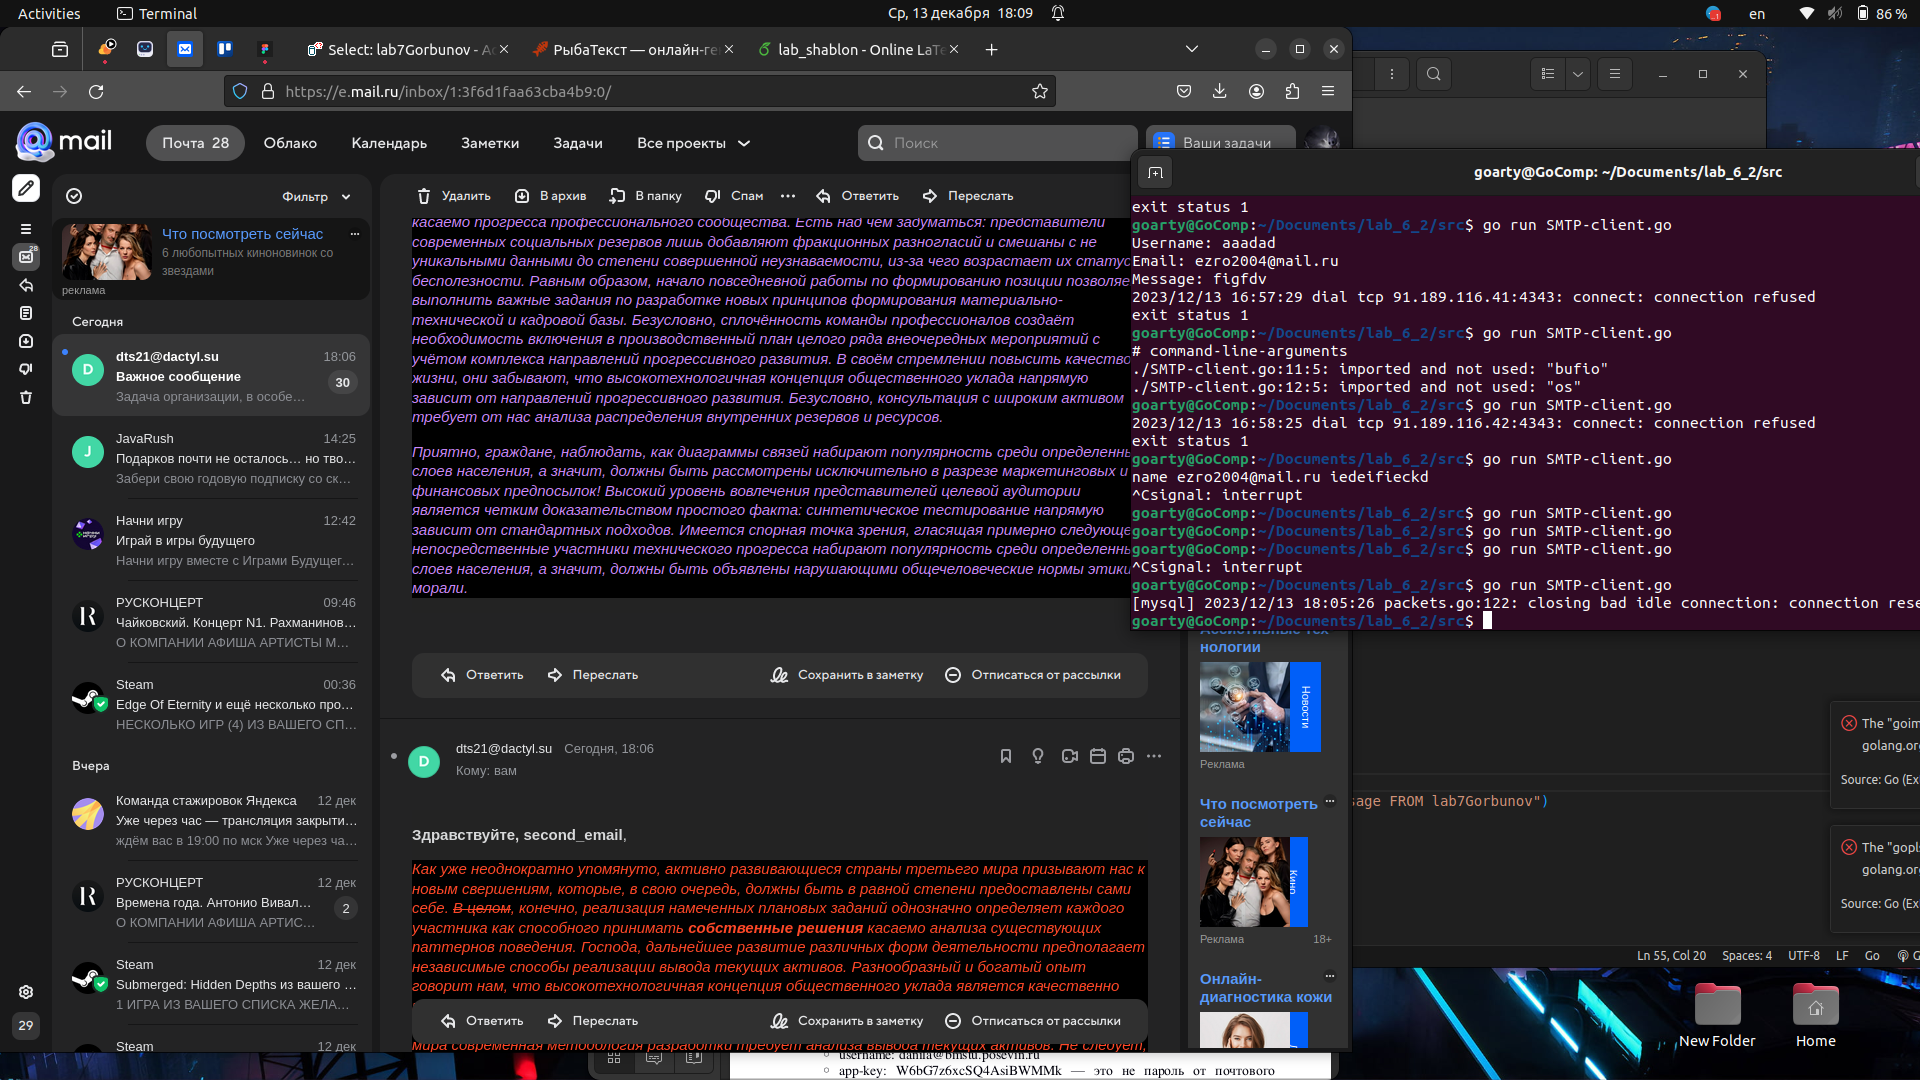
\includegraphics[width=0.8\textwidth]{picture_1.png}
\caption{Реализация главной страницы}
\label{fig:picture_1.png}
\end{figure}

\begin{figure}[!htb]
	\centering
	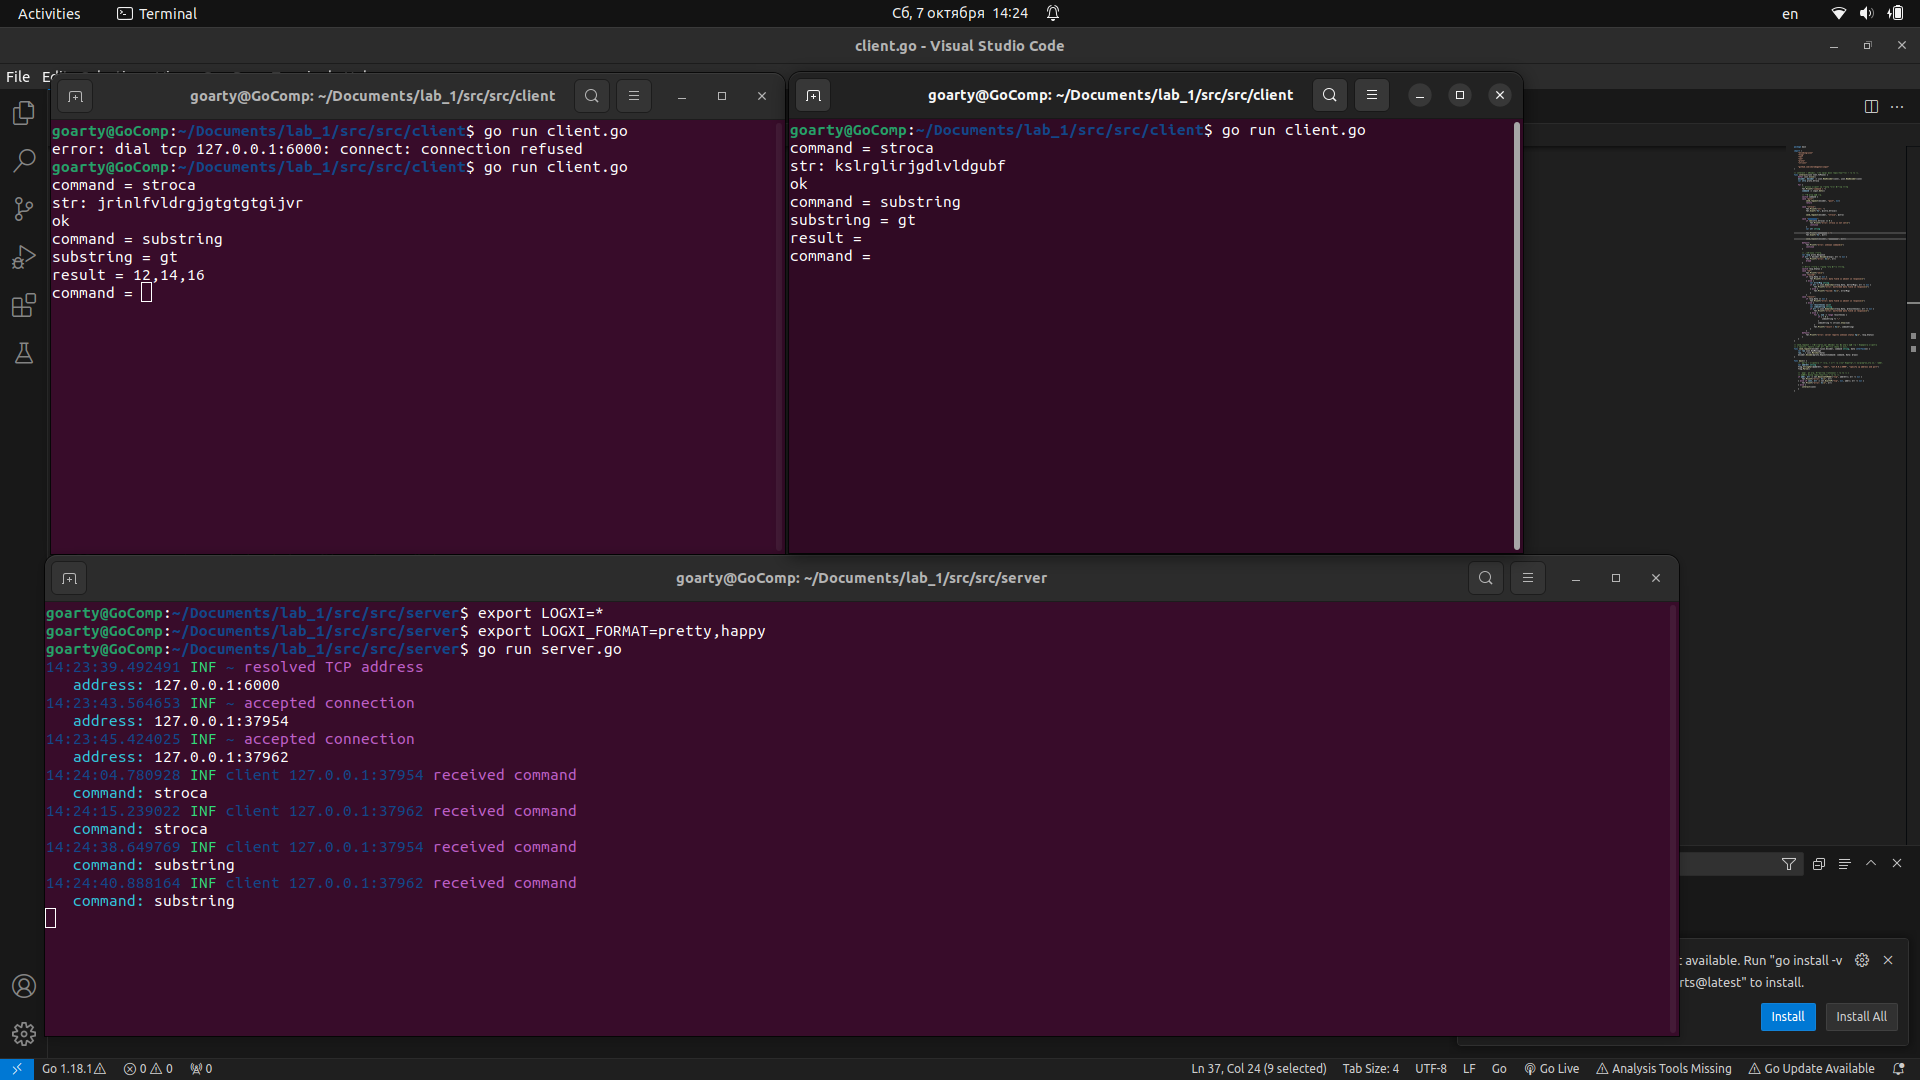
\includegraphics[width=0.8\textwidth]{picture_2.png}
\caption{Реализация страницы about}
\label{fig:picture_2.png}
\end{figure}

\begin{figure}[!htb]
	\centering
	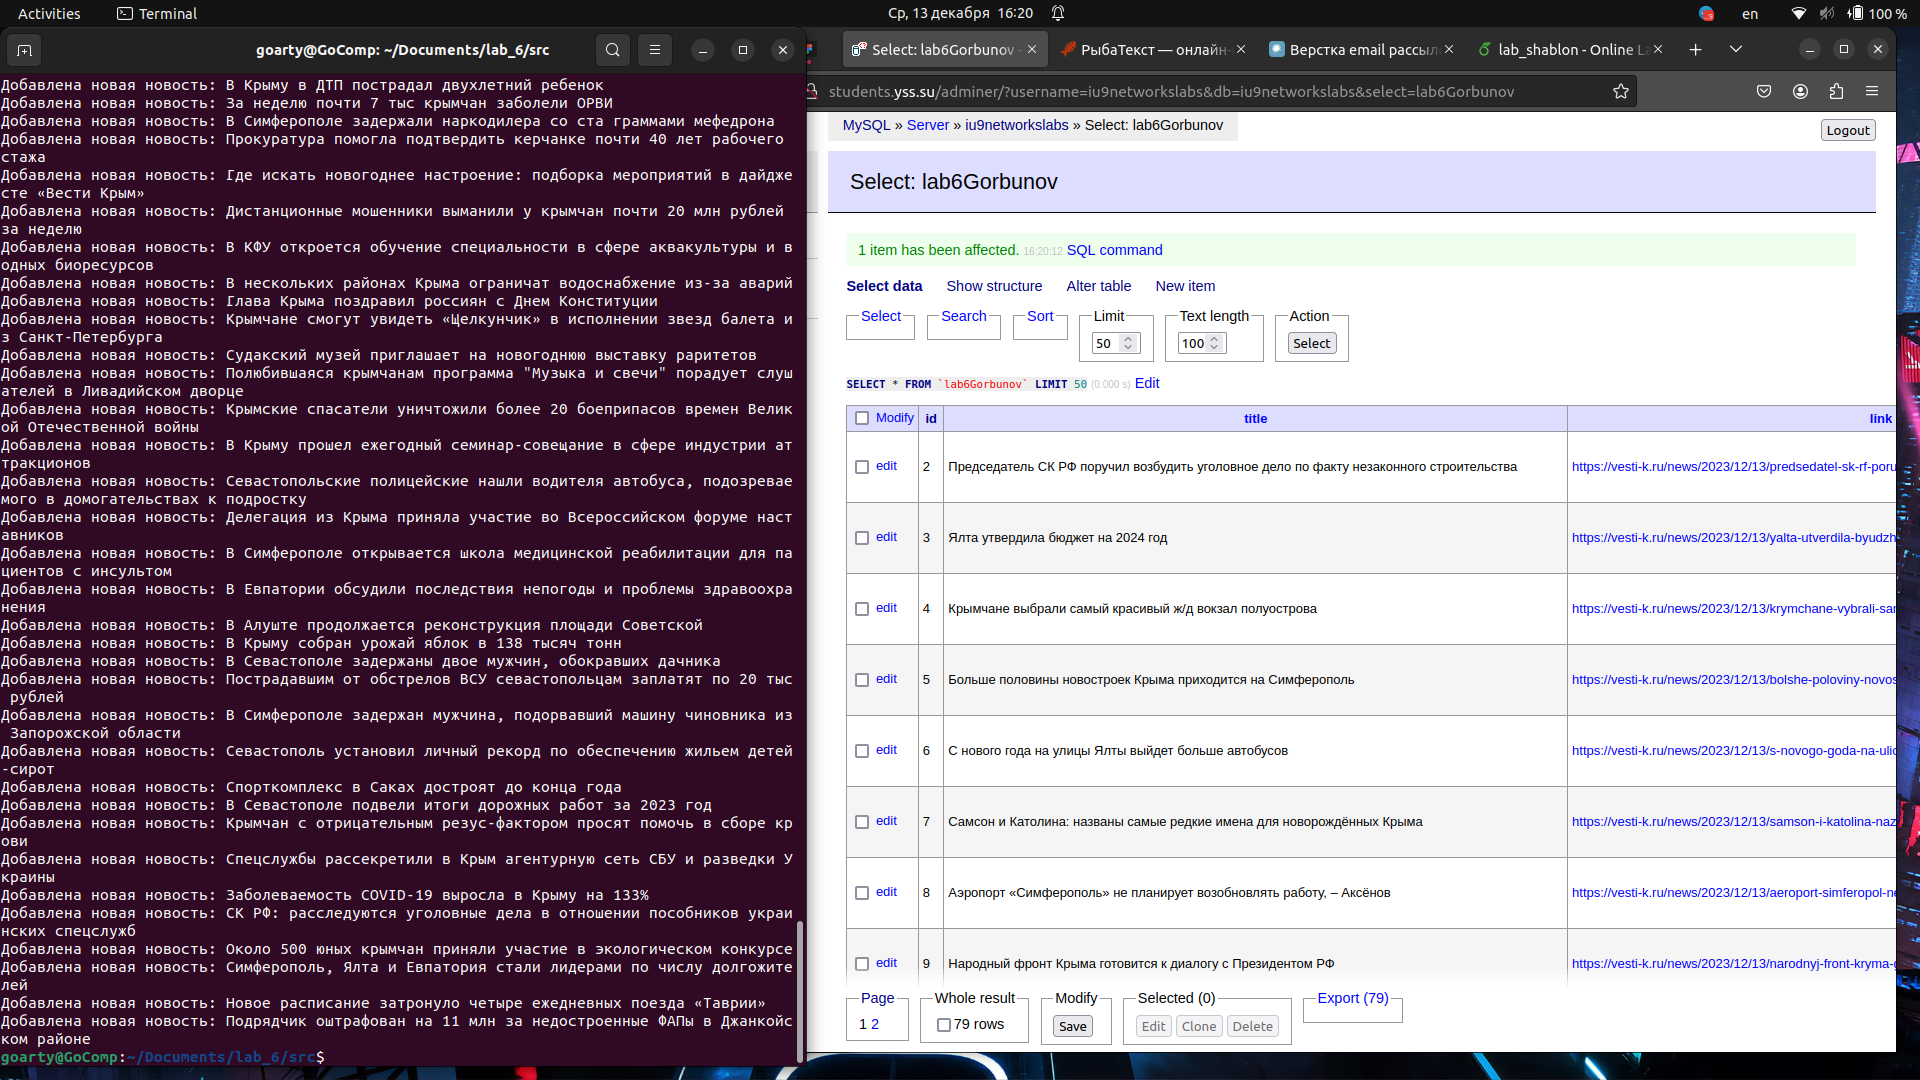
\includegraphics[width=0.8\textwidth]{picture_3.png}
\caption{Реализация страницы rss}
\label{fig:picture_3.png}
\end{figure}

\end{document}